\documentclass{article}

\usepackage{postprocess/context/arxiv}

\usepackage[utf8]{inputenc} % allow utf-8 input
\usepackage[T1]{fontenc}    % use 8-bit T1 fonts
\usepackage{hyperref}       % hyperlinks
\usepackage{url}            % simple URL typesetting
\usepackage{booktabs}       % professional-quality tables
\usepackage{amsfonts}       % blackboard math symbols
\usepackage{nicefrac}       % compact symbols for 1/2, etc.
\usepackage{microtype}      % microtypography
\usepackage{lipsum}		% Can be removed after putting your text content
\usepackage{graphicx}
\usepackage{natbib}
\usepackage{doi}
\usepackage{float}
\usepackage{subcaption}

\title{Causal Discovery Report on Base\_data}

\author{ \href{https://orcid.org/0000-0000-0000-0000}{
\includegraphics[scale=0.06]{postprocess/context/orcid.pdf}\hspace{1mm}Causal Copilot}}

\renewcommand{\headeright}{Technical Report}
\renewcommand{\undertitle}{Technical Report}

\hypersetup{
pdftitle={Causal Discovery Report on Base\_data},
pdfauthor={Causal Copilot},
pdfkeywords={Causal Discovery, Large Language Model, PC},
}

\begin{document}
\maketitle

\begin{abstract}
This report focuses on the causal relationships within the Base\_data dataset, which was subjected to a rigorous analysis using advanced causal discovery techniques. Our methodology involved an initial data preprocessing phase that included statistical examination and exploratory data analysis to address missing values and understand variable distributions. Subsequently, we employed a large language model (LLM) to assist in selecting suitable causal discovery algorithms—namely PC, GES, and DirectLiNGAM—based on the dataset's characteristics. We also fine-tuned hyperparameters through LLM guidance to enhance algorithm performance. Our analysis revealed a complex network of causal influences, particularly identifying significant relationships among variables X0, X1, X2, X5, X6, X4, and X7. Notably, although moderate confidence was found in certain causal links, others exhibited lower reliability, indicating a need for further validation. Our contribution lies in providing a structured approach for causal discovery in unobserved contexts, illustrating both the power and limitations of current methodologies in inferential analyses, and underscoring the necessity for cautious interpretation of causal conclusions in the absence of domain knowledge.
\end{abstract}

\keywords{Causal Discovery, Large Language Model, PC}

\raggedbottom
\section{Introduction}
Causal discovery is a critical area of research that aims to identify the underlying causal relationships among variables in a given dataset. In the absence of prior knowledge about the dataset, the analysis becomes particularly challenging yet intriguing, as it requires the application of various statistical and computational techniques to infer potential causal structures. This report presents an in-depth investigation into the dataset, employing state-of-the-art causal discovery algorithms to uncover meaningful relationships and elucidate the complexities within the data. The findings from this analysis will not only contribute to a better understanding of the interdependencies present but also provide valuable insights for future research and practical applications.

\section{Dataset Descriptions and EDA}
The following is a preview of our original dataset.

\begin{table}[H]
    \centering
    \caption{Dataset Preview}
    \begin{tabular}{rrrrrrrr}
\toprule
 X0 &  X1 &  X2 &  X3 &  X4 &  X5 &  X6 &  X7 \\
\midrule
  1 &   1 &   0 &   1 &   1 &   0 &   0 &   1 \\
  1 &   0 &   0 &   0 &   1 &   1 &   1 &   0 \\
  1 &   0 &   1 &   1 &   1 &   0 &   0 &   1 \\
  0 &   1 &   0 &   0 &   1 &   1 &   1 &   0 \\
  0 &   0 &   0 &   0 &   1 &   1 &   1 &   1 \\
\bottomrule
\end{tabular}

\end{table}

\subsection{Data Properties}
We employ several statistical methods to identify data properties.

The shape of the data, data types, and missing values are assessed directly from the dataframe.
Linearity is evaluated using Ramsey’s RESET test, followed by the Benjamini \& Yekutieli procedure for multiple test correction.
Gaussian noise is assessed through the Shapiro-Wilk test, also applying the Benjamini \& Yekutieli procedure for multiple test correction.
Time-Series and Heterogeneity are derived from user queries.

Properties of the dataset we analyzed are listed below.

\begin{table}[H]
    \centering
    \caption{Data Properties}

        \begin{tabular}{rrrrrrr}
            \toprule
            Shape ($n$ x $d$) & Data Type & Missing Value & Linearity & Gaussian Errors & Time-Series & Heterogeneity \\
            \midrule
            (1500, 8)   & Continuous & False & False & False & False & False \\
            \bottomrule
        \end{tabular}
        
\end{table}


\subsection{Distribution Analysis}
The following figure shows distributions of different variables. The orange dash line represents the mean, 
and the black line represents the median. Variables are categorized into three types according to their distribution characteristics.

\begin{figure}[H]
\centering
\includegraphics[width=\linewidth]{postprocess/test_data/20241007_184921_base_nodes8_samples1500/output_graph/eda_dist.jpg}
\caption{\label{fig:dist}Distribution Plots of Variables}
\end{figure}

\begin{itemize}
\item Slight left skew distributed variables: None
\item Slight right skew distributed variables: None
\item Symmetric distributed variables: X0, X1, X2, X3, X4, X5, X6, X7
\end{itemize}

\subsection{Correlation Analysis}

\begin{minipage}[t]{0.5\linewidth}
    In this analysis, we will categorize the correlation statistics of features in the dataset into three distinct categories: Strong correlations ($r>0.8$), Moderate correlations ($0.5<r<0.8$), and Weak correlations ($r<0.5$).

\begin{itemize}
\item Strong Correlated Variables: None
\item Moderate Correlated Variables: None
\item Weak Correlated Variables: None
\end{itemize}
\vfill
\end{minipage}
\hfill
\begin{minipage}[t]{0.5\linewidth}
    \begin{figure}[H]
        \centering
        \vspace{-1.5cm}
        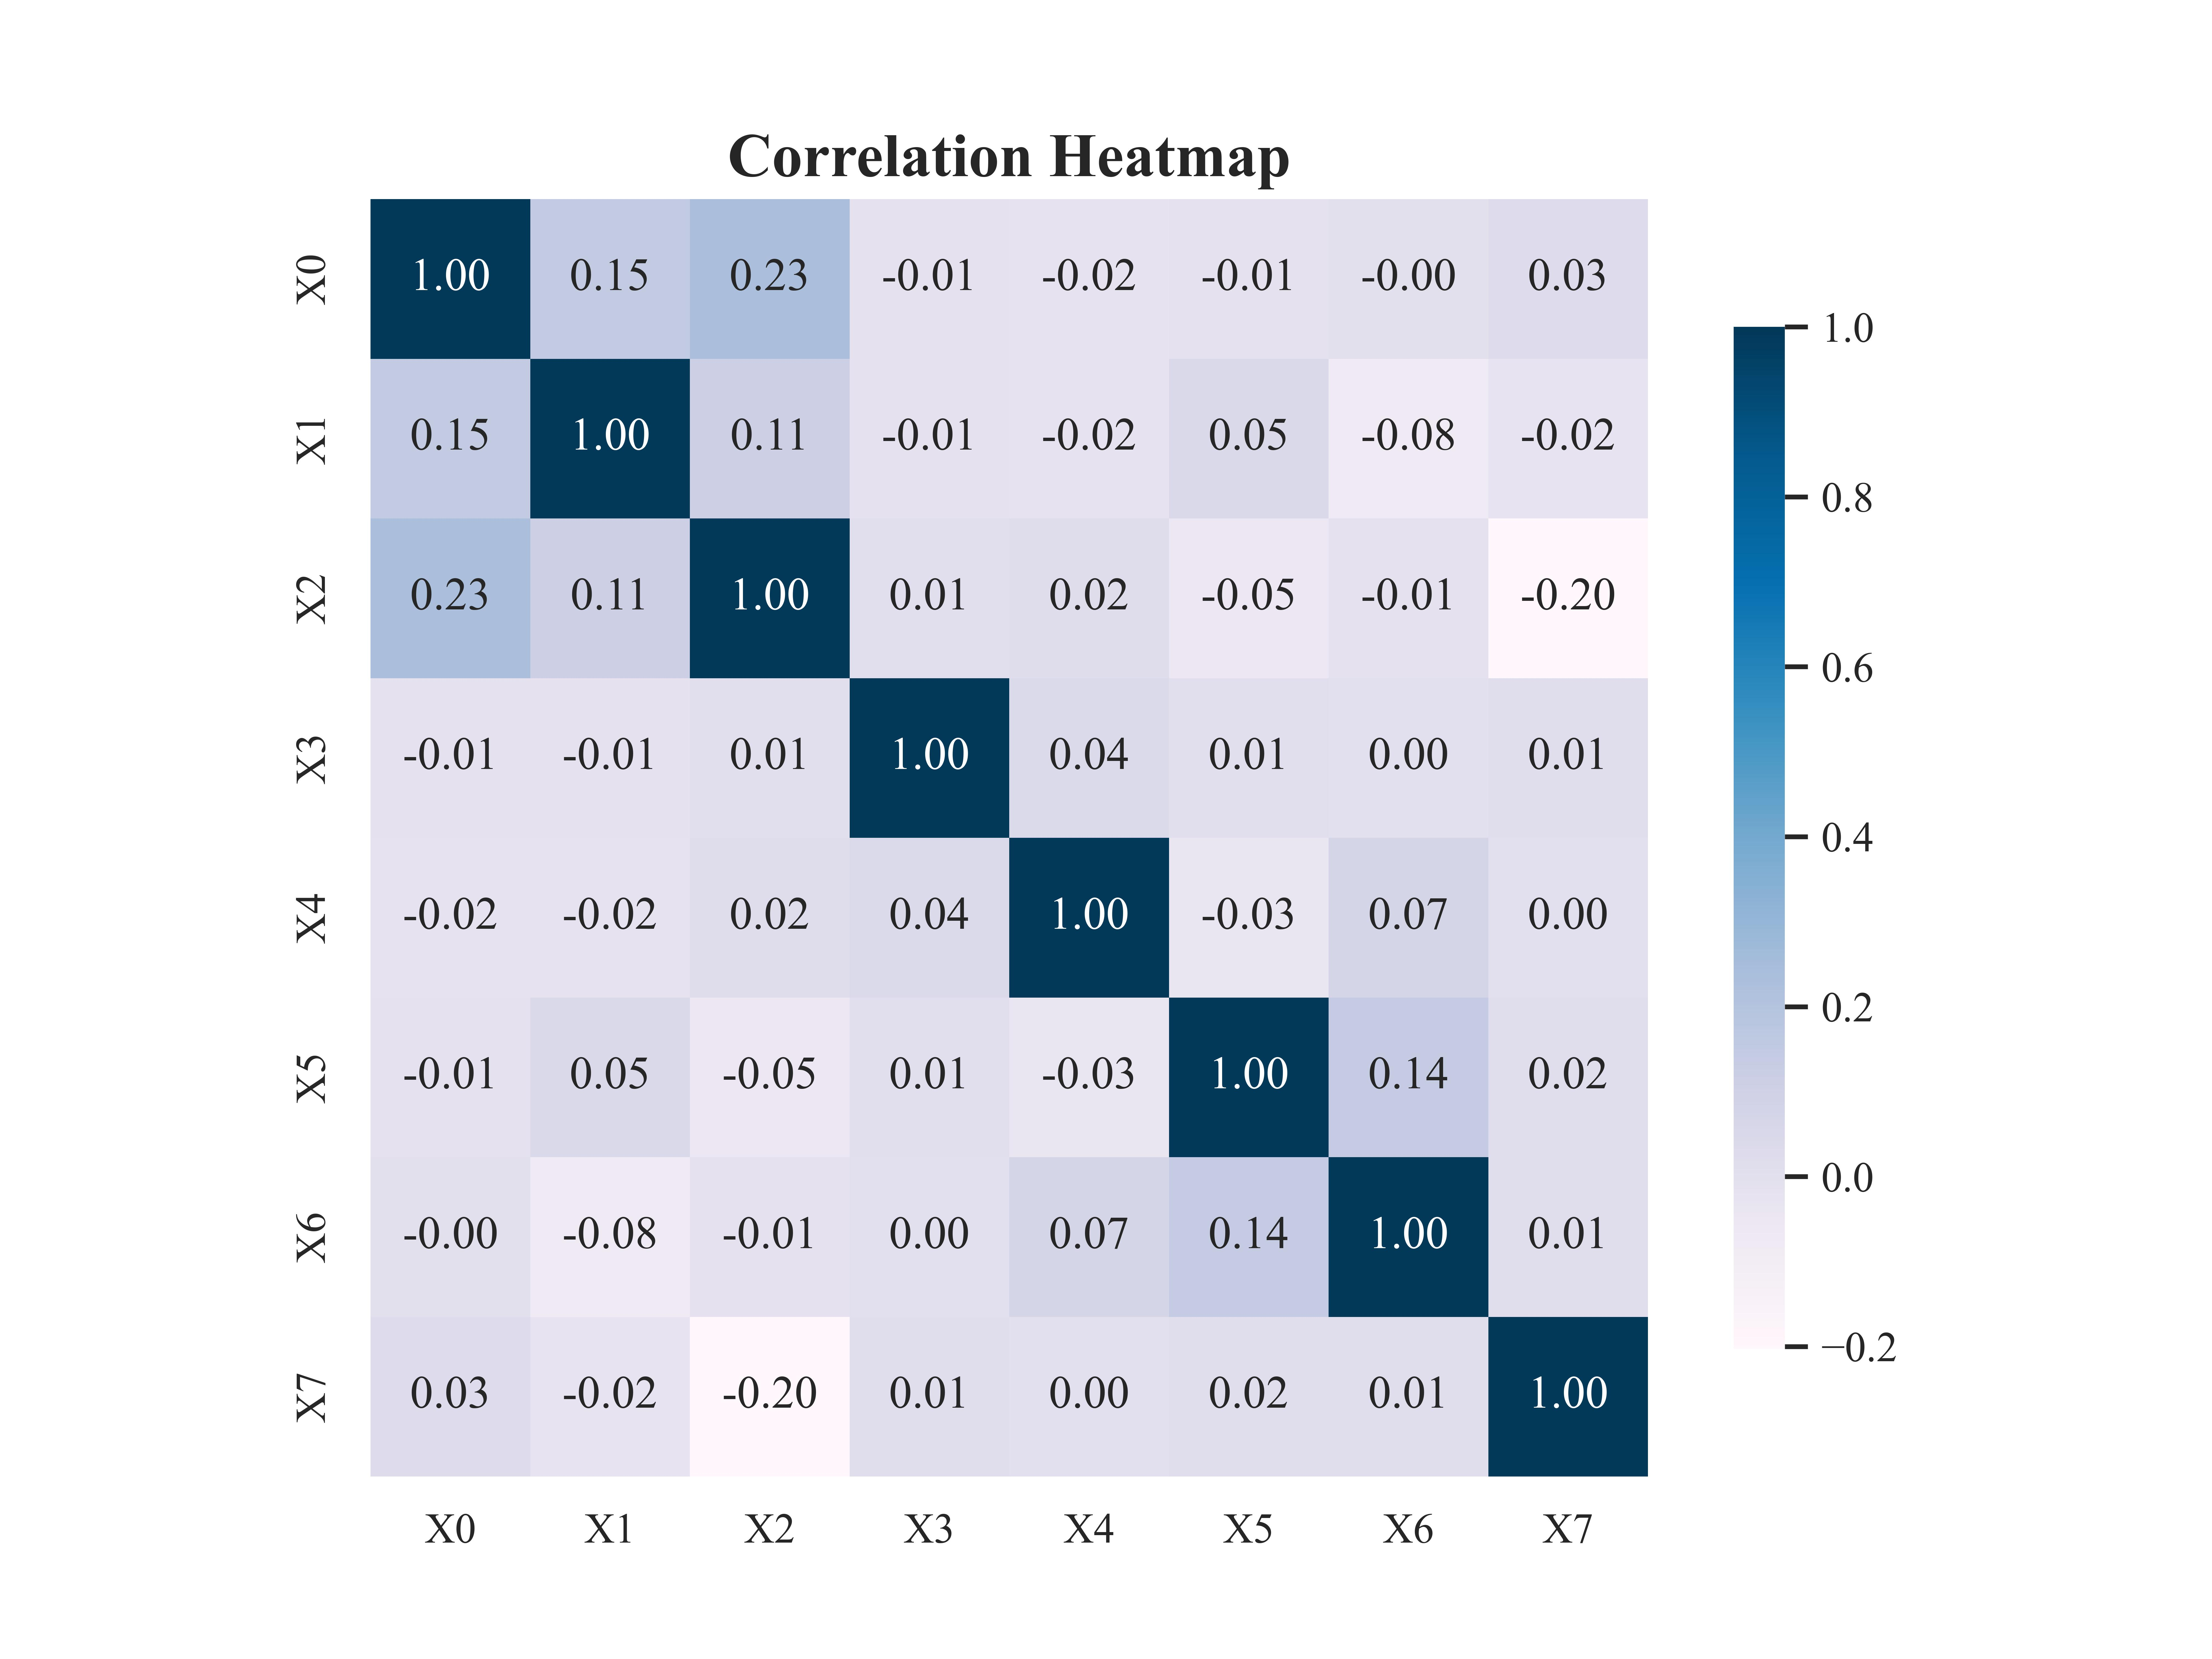
\includegraphics[width=\linewidth]{postprocess/test_data/20241007_184921_base_nodes8_samples1500/output_graph/eda_corr.jpg}
        \caption{\label{fig:corr}Correlation Heatmap of Variables}
    \end{figure}
\end{minipage}

\section{Discovery Procedure}

        In this section, we provide a detailed description of the causal discovery process implemented by Causal Copilot. 
        We also provide the chosen algorithms and hyperparameters, along with the justifications for these selections.

        \subsection{Data Preprocessing}
        In this initial step, we preprocessed the data and examined its statistical characteristics. 
        This involved cleaning the data, handling missing values, and performing exploratory data analysis to understand distributions and relationships between variables.
                
        \subsection{Algorithm Selection assisted with LLM}
        Following data preprocessing, we employed a large language model (LLM) to assist in 
        selecting appropriate algorithms for causal discovery based on the statistical characteristics of the dataset and relevant background knowledge. 
        The top three chosen algorithms, listed in order of suitability, are as follows:   
        
        \begin{itemize}

        
                        \item \textbf{PC}:
                        \begin{itemize}
                            \item \textbf{Description}: The PC algorithm is a constraint-based method that learns the structure of a causal graph from data by testing conditional independencies between variables. It constructs a directed acyclic graph (DAG) representing the causal relationships.
                            \item \textbf{Justification}: Given the dataset's large sample size, PC is efficient for discovering causal structures when all relevant variables are observed. The assumption of sufficient data allows it to operate effectively despite non-linearities.
                        \end{itemize}

                         
                        \item \textbf{GES}:
                        \begin{itemize}
                            \item \textbf{Description}: Greedy Equivalence Search (GES) is a score-based causal discovery algorithm that identifies the optimal causal structure by navigating the space of equivalence classes of Directed Acyclic Graphs (DAGs).
                            \item \textbf{Justification}: GES is suitable due to the dataset's characteristics: with no missing values and a large sample size, it can effectively handle the non-linear relationships present in a more complex search space efficiently.
                        \end{itemize}

                         
                        \item \textbf{DirectLiNGAM}:
                        \begin{itemize}
                            \item \textbf{Description}: DirectLiNGAM improves the original LiNGAM framework by introducing an efficient stepwise linear regression approach to directly estimate the causal order.
                            \item \textbf{Justification}: Although DirectLiNGAM assumes linear relationships, its effectiveness in handling non-Gaussian errors can still be leveraged in this dataset, making it a valuable option for causal discovery.
                        \end{itemize}

                         
                    \end{itemize}
                    

        \subsection{Hyperparameter Values Proposal assisted with LLM}
        Once the algorithms were selected, the LLM aided in proposing hyperparameters 
        for the [ALGO] algorithm, which are specified below:
        
        \begin{itemize}

        
                        \item \textbf{alpha}:
                        \begin{itemize}
                            \item \textbf{Value}: 0.1
                            \item \textbf{Explanation}: Given that the dataset is relatively large (1500 samples) and does not exhibit predominantly linear relationships, a slightly higher alpha value of 0.1 is suggested to avoid missing true causal relationships. This balances the need for detecting edges without being overly conservative.
                        \end{itemize}

                         
                        \item \textbf{indep\_test}:
                        \begin{itemize}
                            \item \textbf{Value}: fisherz
                            \item \textbf{Explanation}: Although Fisher's Z test assumes normality and linear relationships, it is still appropriate given that the data is continuous even if it does not meet all assumptions. As this dataset features continuous data types, Fisher's Z is the best method among the alternatives since chi-squared tests are not suitable for continuous data without discretization.
                        \end{itemize}

                         
                        \item \textbf{depth}:
                        \begin{itemize}
                            \item \textbf{Value}: -1
                            \item \textbf{Explanation}: Setting the depth to -1 allows the algorithm to explore all possible relationships between the variables without restricting the depth of the search. This is justified given the dataset's characteristics, as there are no known complexities that would necessitate limiting the search.
                        \end{itemize}

                         
                    \end{itemize}
                    

        
        This structured approach ensures a comprehensive and methodical analysis of the causal relationships within the dataset.
        

\section{Results Summary}

\begin{figure}[H]
    \centering
    \begin{subfigure}{0.45\textwidth}
        \centering
        \vspace{-0.5cm}
        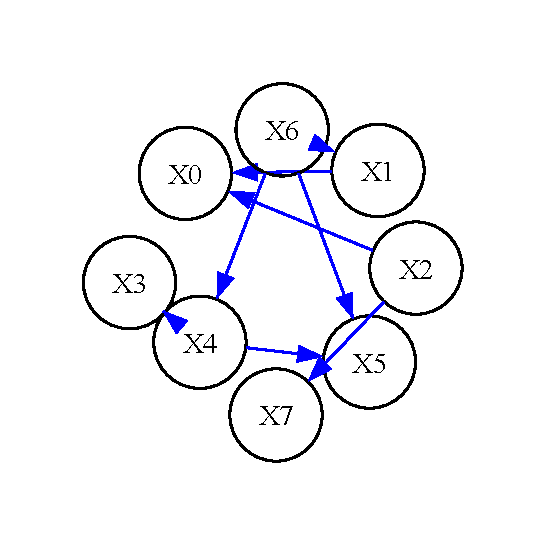
\includegraphics[width=\linewidth]{postprocess/test_data/20241007_184921_base_nodes8_samples1500/output_graph/true_graph.pdf}
        \vfill
        \caption{True Graph}
        \label{fig:sub1}
    \end{subfigure}
    \hspace{0.04\textwidth}
    \begin{subfigure}{0.45\textwidth}
        \centering
        \vspace{-0.5cm}
        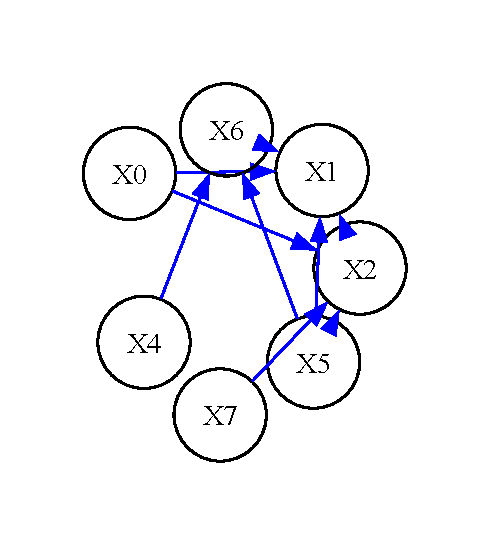
\includegraphics[width=\linewidth]{postprocess/test_data/20241007_184921_base_nodes8_samples1500/output_graph/initial_graph.pdf}
        \vfill
        \caption{Initial Graph}
        \label{fig:sub2}
    \end{subfigure}
    \caption{Graphs Comparison of PC}
    \label{fig:main}
\end{figure}

The above are the true graph and the result graph produced by our algorithm.

The causal relationships among the variables illustrate a complex network of influence where X0 serves as a precursor to both X1 and X2, indicating that changes in X0 can directly affect these subsequent variables. Additionally, X2 has a causative effect on X1, suggesting that the dynamics involving X0 and X2 play a significant role in shaping the behavior of X1. Furthermore, X5 emerges as a pivotal variable, exerting influence over X1, X2, and X6, thereby linking these variables in a chain of causation that underscores the interconnectedness of their relationships. The causation extends to X6 affecting X1, establishing an additional layer of influence from X5 through X6 to X1. Meanwhile, X4 impacts X6, positioning it as a potential regulator within the system. Finally, X7 influences X2, indicating that X2's response may also be shaped by external factors represented by X7, which adds complexity to the causal web. Overall, each variable plays a distinct role, contributing to the network of cause and effect that characterizes this system.

\subsection{Graph Reliability Analysis}

\begin{figure}[H]
        \centering
        \vspace{-0.5cm}
        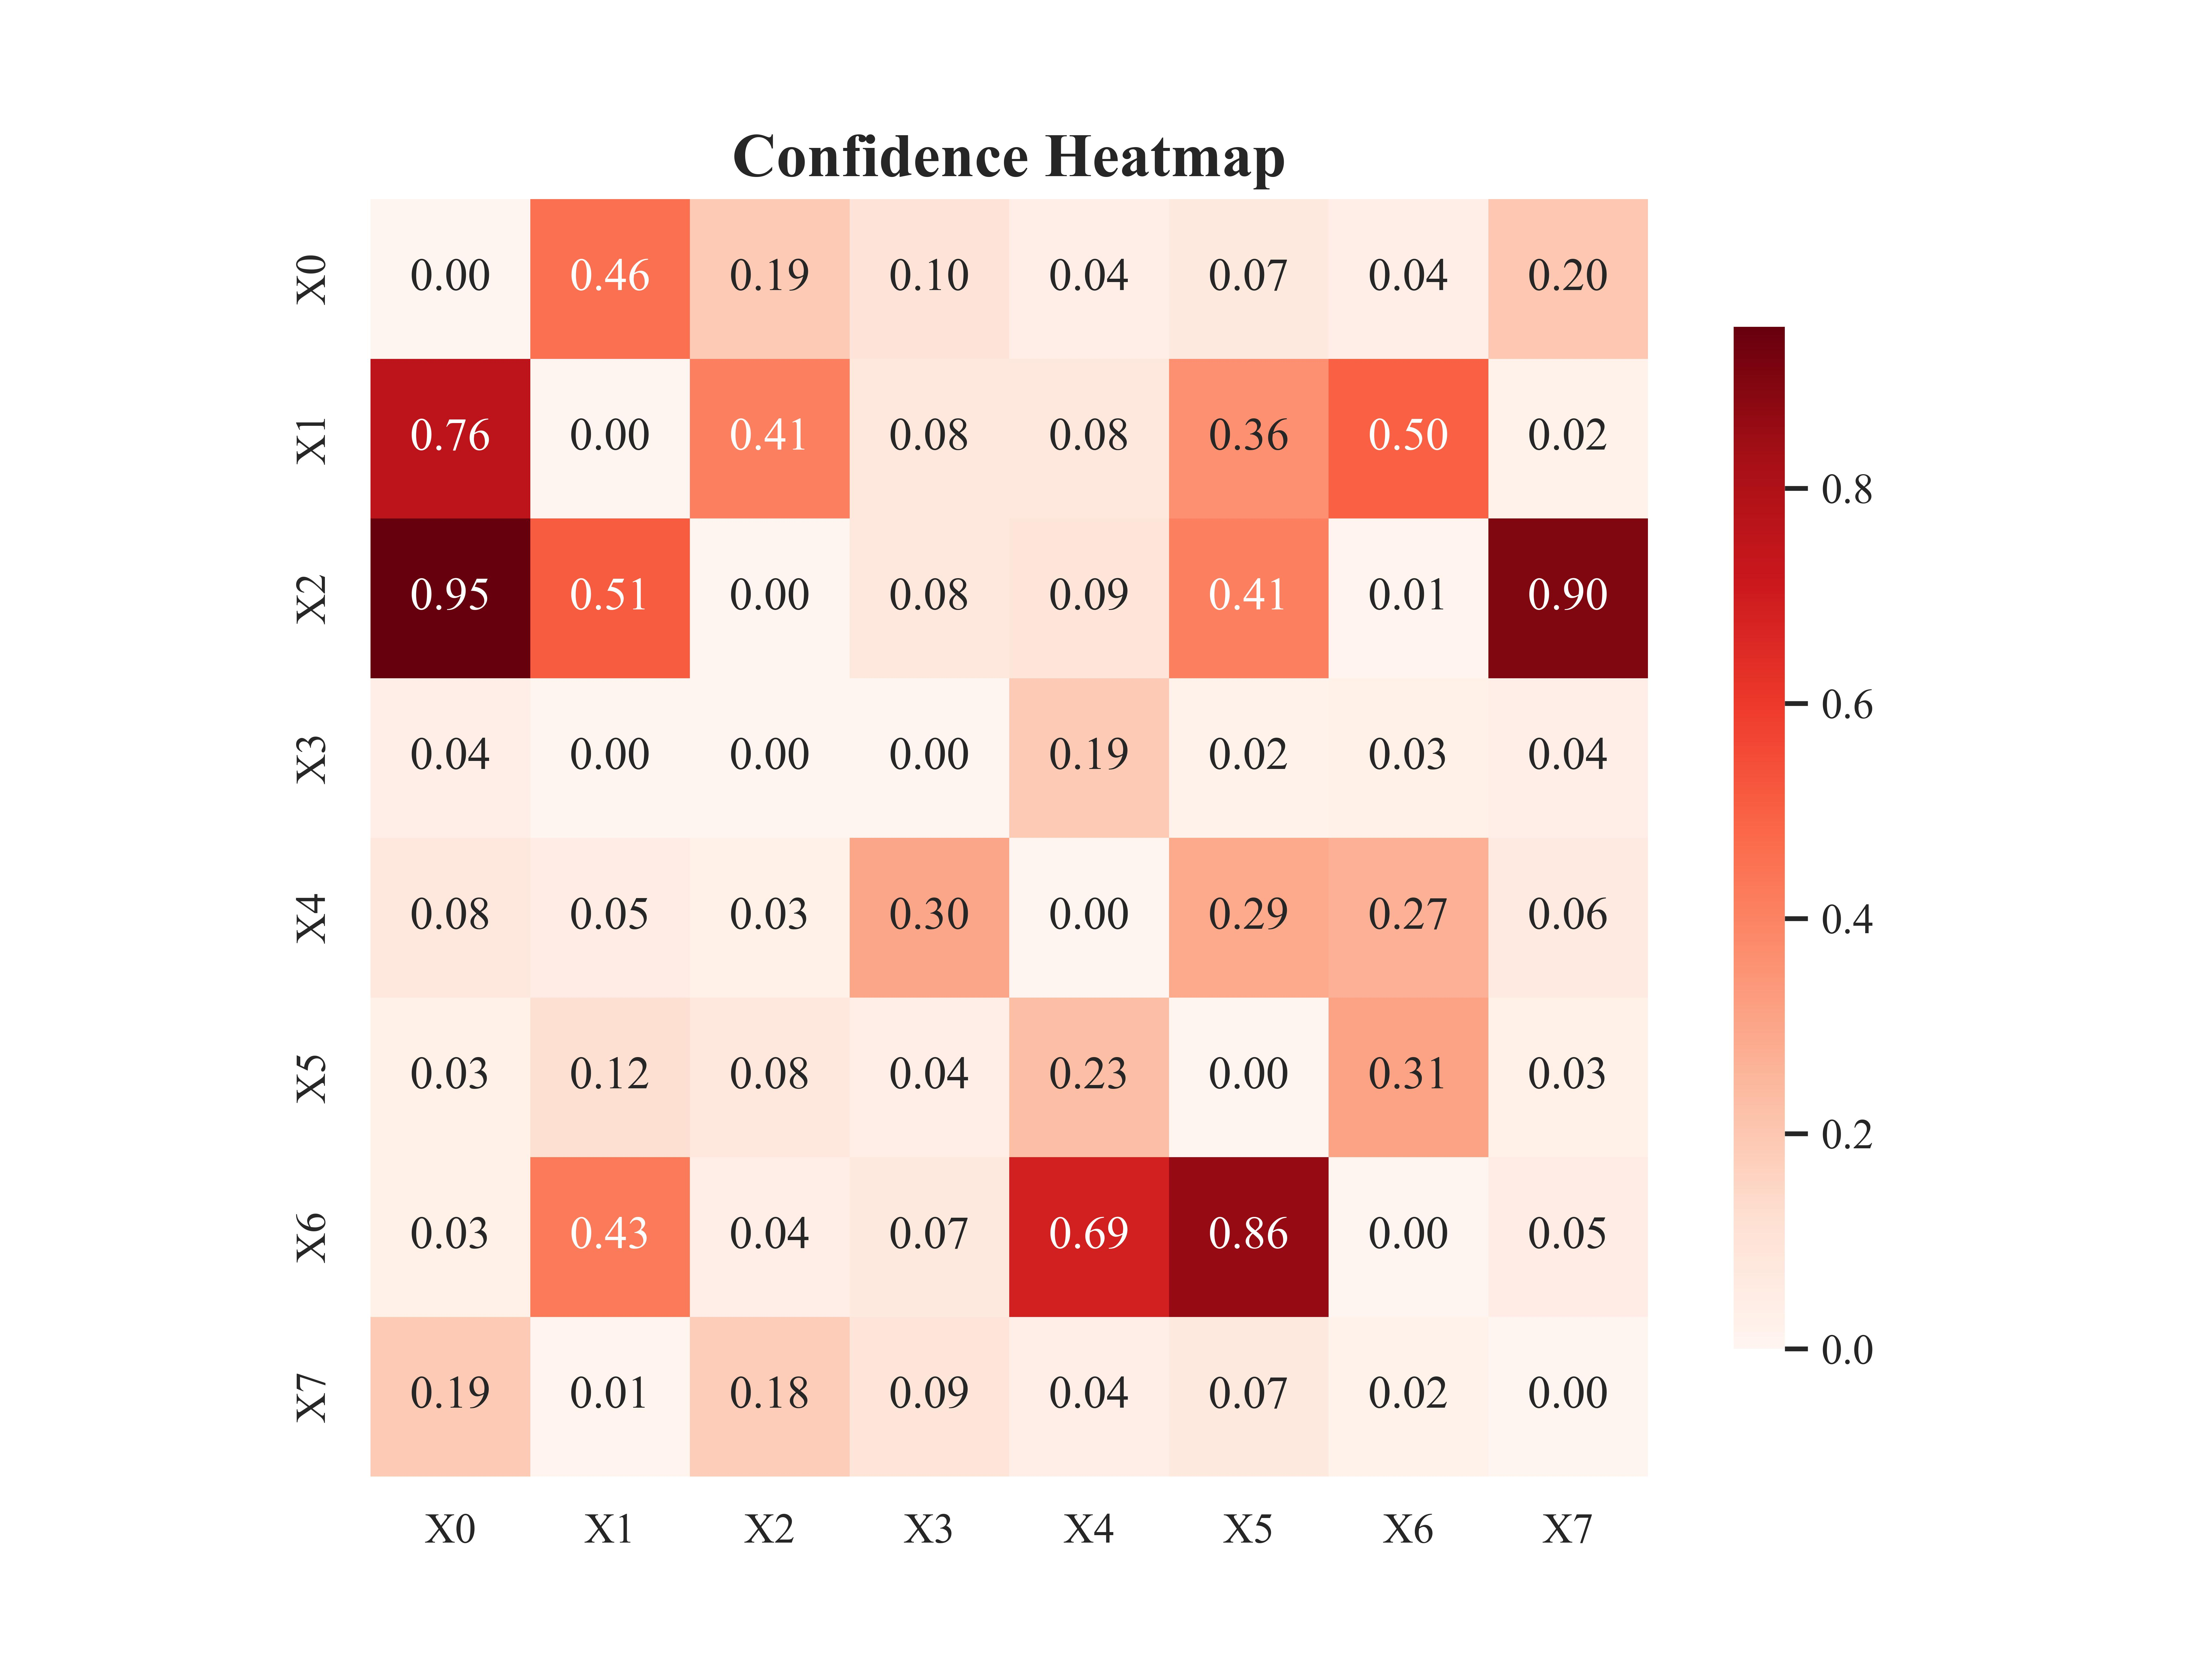
\includegraphics[width=0.8\linewidth]{postprocess/test_data/20241007_184921_base_nodes8_samples1500/output_graph/confidence_heatmap.jpg}
        \caption{Reliability Graph}
        \label{fig:sub3}
\end{figure}

Based on the confidence probability heatmap and background knowledge, we can analyze the reliability of our graph.

From the statistics perspective, we have moderate confidence to believe that these edges exist: X2 $\rightarrow$ X1 (bootstrap probability of 0.51) and X6 $\rightarrow$ X1 (bootstrap probability of 0.43), indicating a significant likelihood of these causal relationships. However, we have low confidence in the existence of the following edges due to their lower bootstrap probabilities: X0 $\rightarrow$ X1 (0.46), X4 $\rightarrow$ X6 (0.27), X5 $\rightarrow$ X1 (0.12), X5 $\rightarrow$ X2 (0.08), X5 $\rightarrow$ X6 (0.31), and X7 $\rightarrow$ X2 (0.18), suggesting that these relationships may not be robust.

However, based on the expert knowledge, since we have no specific background information regarding the variables in question, we cannot definitively assert the existence or non-existence of any causal relationships. The absence of background knowledge implies that we cannot corroborate or dispute any of the statistical findings with domain expertise.

Therefore, the result of this causal graph is somewhat unreliable. The moderate to low confidence levels indicated by the bootstrap probabilities suggest that many proposed edges may not represent true causal relationships, highlighting the need for further investigation and validation before drawing concrete conclusions regarding these variables.

\end{document}